\subsection{Communication Message Broker}

A communication framework supports the \flux\ hierarchical job model
by establishing a {\em comms session} to contain each \flux\ instance
and provide a foundation for the distributed components upon which
\flux\ will be built.
This framework enables secure, scalable communication
within a comms session, limits communication between sessions,
and allows new comms sessions to be created, resized, destroyed,
and monitored by existing ones in a parent-child relationship.

We have built a primitive prototype of the \flux\ communications framework
using \zMQ~\cite{ZMQGuide} which we can launch within a
Slurm~\cite{Jette02slurm} job.
\zMQ\ provides the ability to manipulate opaque,
multipart messages, and carry them across various transports, including
TCP and Pragmatic General Multicast (PGM)~\cite{rfc3208}
using a socket-like API.
\zMQ\ provides abstractions that ease implementation of common
messaging patterns including {\em request-reply}, {\em publish-subscribe},
and {\em push-pull}.
\zMQ\ can be used to build applications or custom message brokers.

Our prototype consists of a distributed Comms Message Broker (CMB)
daemon which runs on each node of a comms session, interconnected using
three persistent overlay network planes:
\begin{enumerate}
\item{a PGM {\em publish-subscribe} bus for events}
\item{a TCP {\em dealer-router} (advanced {\em request-response})
tree for upstream RPCs and reductions
similar to those enabled by MrNet~\cite{mrnet}}
\item{a secondary TCP {\em dealer-router} tree for downstream RPCs.}
\end{enumerate}

\begin{figure}
\centering
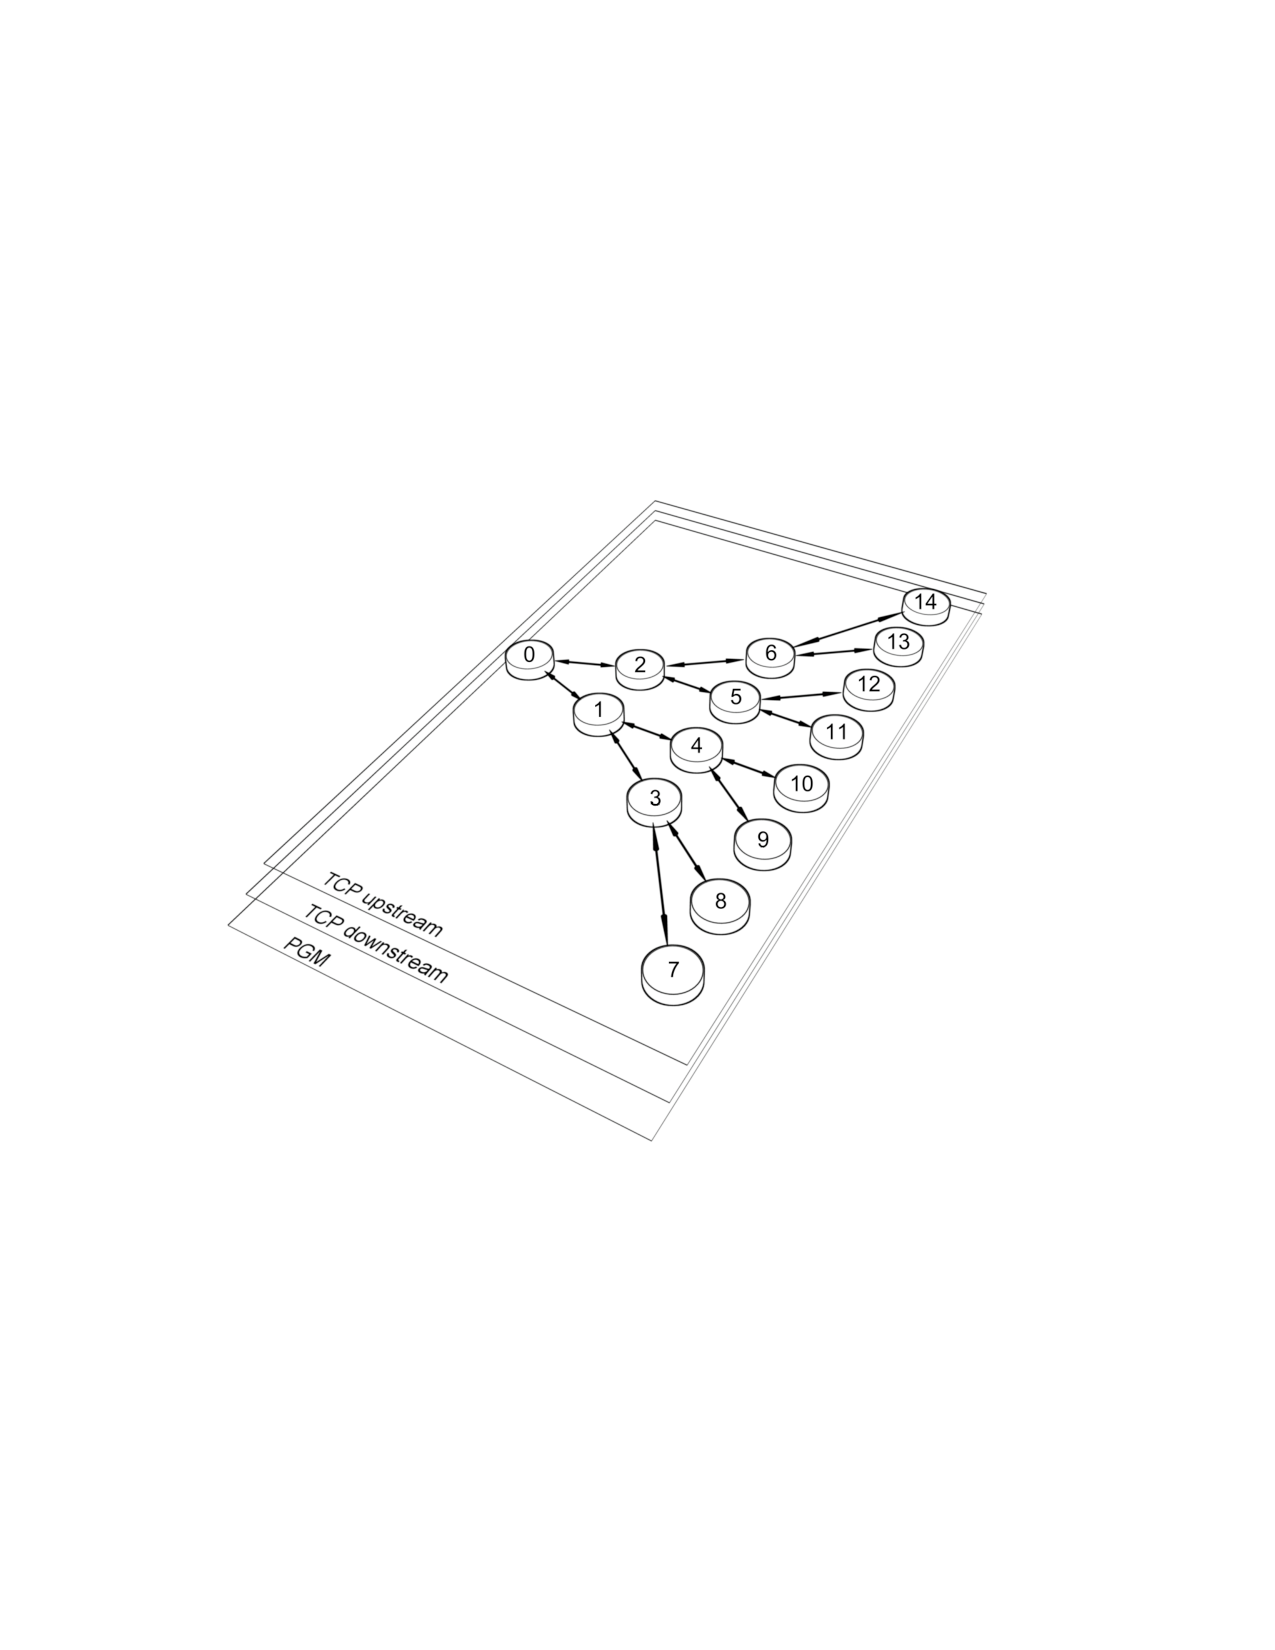
\includegraphics[trim=5.0cm 8.0cm 5.0cm 8.0cm,scale=0.5]{B_Tree_4Layer_BW}
\caption{A comms session consists of daemons interconnected using
three persistent overlay network planes:
a TCP {\em dealer-router} tree for upstream RPCs and reductions,
a TCP {\em dealer-router} tree for downstream RPCs, and
a PGM {\em publish-subscribe} bus for events.
Although a binary tree is pictured, the RPC planes can be launched in
any tree shape for testing or to tune performance.
%Flat, degenerate, {\em k}-ary for several values of {\em k}, and
%binomial have been tested.
}
\label{fig:commswireup}
\end{figure}

The comms session wire-up is depicted in Figure~\ref{fig:commswireup}.
Each message plane implements reliable, in-order message delivery, and
can self-heal when nodes other than the root node fail.
Security and comprehensive fault-tolerance are not yet implemented,
but are near-term design topics.

The CMB allows us to experiment with loosely coupled distributed services
while reusing the underlying message routing framework.  Various comms
services have been implemented as CMB plugins.  Plugins currently exist for
the services listed in Table~\ref{tab:cmbplugins}.
Each embodies an active topic for study and experimentation by the \flux\ team.

\begin{table}
\centering
\caption{CMB plugins implement basic building blocks for \flux\ and
potentially other applications.  These are the plugins we have prototyped
thus far, representing a wide range of design maturity.  Each embodies an
active topic for study and experimentation by the \flux\ team.}
\begin{tabular}{|l|p{9cm}|}\hline
\textbf{Plugin} & \textbf{Description} \\
\hline
heartbeat & A periodic heartbeat event multicast across the comms
	session synchronizes background activity to reduce scheduling jitter.\\
\hline
live & Each tree node receives heartbeat-synchronized {\em hello}
	messages from its children.  After a configurable number of missed
	messages, a liveness event is issued for a dead child.\\
\hline
log & Log messages are reduced and filtered before being placed in
	a log file at the session root.  A circular debug buffer
	provides log context in response to a fault event.\\
\hline
mon & Lua scripts stored in the KVS activate heartbeat-synchronized sampling.
	Samples are reduced and stored in the KVS.\\
\hline
group & \flux\ groups define and manage collection of processes that can
	participate in collective operations.\\  
\hline
barrier & Collective barriers provide synchronization across \flux\ groups. \\
\hline
kvs & A distributed key-value store provides a scalable scratchpad
	for \flux\ and other tools operating within the comms session.\\
\hline
wrexec & Remote processes can be launched in bulk, monitored,
	receive signals, and have standard I/O captured in the KVS.\\
\hline
resrc & Resources are enumerated in the KVS and allocated
	when the scheduler runs a lightweight job. \\
\hline
sched & Lightweight job requests are queued in the KVS, assigned
	resources, and launched. \\
\hline
\end{tabular}
\label{tab:cmbplugins}
\end{table}

In addition to CMB plugins, external programs can communicate with the CMB
via a UNIX domain socket.  A {\tt flux} utility wraps up two dozen or so
modular subcommands used to interact with and test the CMB plugins.

All CMB messages have a uniform multi-part message format consisting of
a {\em tag frame} and a {\em JSON~\cite{rfc4627} frame}.  The tag frame identifies the
message recipient using a hierarchical name space.  For example a message
sent to the tag {\em kvs.put} is routed to the {\em kvs} plugin, and internally
to its handler for {\em put}.  The tag frame format is identical to
\zMQ's {\em publish-subscribe} topic string format, thus CMB messages
have the same format on all three overlay networks.
The message payload is contained in the free-form JSON frame.

Most requests are routed via the upstream request overlay network
and utilize the \zMQ\ {\em dealer-router} pattern's built-in source routing
scheme for returning optional replies to the sender over the same network.
Requests are routed to the first plugin encountered in the tree that claims
the tag, or are negatively acknowledged at the root.  This enables plugins
to be loaded at a variable tree depth to tune its level of distribution
or conserve node resources for application workloads toward the leaves.
Reductions are simply requests that are aggregated and retransmitted between
instances of a plugin, traversing upstream.

Explicit rank-addressing is available for requests that must target a
specific CMB instance by rank.  The rank is prepended to the tag frame,
and routing tables are consulted at each hop to determine which overlay
to use to reach the destination.  If the downstream overlay is selected,
the routing table entry determines which branch of the tree to use.
In this manner an RPC can take place between any two ranks in the session.

As our designs and prototypes for basic \flux\ building blocks evolve,
the CMB evolves to provide necessary services.  For example, the CMB API
now has both C and Lua~\cite{LuaBook}  bindings and a custom event reactor interface in
response to the experience of meeting a recent milestone to launch an
MPI job internally and co-locate a distributed debugger.  Some of the building
blocks built on CMB services, such as the key-value store plugin described
in the next section, are independently undergoing design iteration.
We expect to continue evolving the CMB prototype for several more months until
our design has reached stability and we build a production-level \flux\ 
communication framework.
